%summary for IMA

\documentclass[french]{article}
\usepackage[utf8]{inputenc}
\usepackage[T1]{fontenc}
\usepackage{babel}
\usepackage{lmodern}
\usepackage{graphicx}
\usepackage{tikz}
\usetikzlibrary{arrows}

\usepackage{amsmath}
\usepackage{amsfonts}
\usepackage{mathrsfs}

\usepackage{float}

\title{Ima}
\date{}
\author{L3 RI}


\begin{document}
\maketitle
\tableofcontents
\newpage

\section{Introduction}
On considère des images en niveaux de gris. À chaque pixel d'une image
on associe donc une valeur dans ${0\dots255}$
\subsection{Histogramme}
L'histogramme d'une image donne des informations sur la densité de
chaque valeur.
\paragraph{Définition} L'histogramme d'une image $I$ est une fonction
discrète qui associe à chaque valeur d’intensité le nombre de pixels
prenant cette valeur.
$$
\begin{array}{rccl}
h_t : & {0\dots255} & \to & \mathbb{N} \\
 & n & \mapsto & \text{Card}\left\{(x,y) | I(x,y) = n\right\}\\
\end{array}
$$
\subparagraph{Remarque} Si on a une image de taille $p\times q$ alors
$\sum_{n = 0}^{255} h_t(n)= p*q$

\subparagraph{Propriété} L'histogramme d'une image et de sa translation
sont les mêmes. Ce n'est donc \emph{pas une caractéristique de l'image}.

\paragraph{Interprétation} Si l'histogramme est condensé sur les valeurs
faibles (resp. sur les fortes) alors l'image est \emph{sous-exposée} (resp.
\emph{surexposée}).

\paragraph{Égalisation} On peut normaliser un histogramme condensé en
étalant ces valeurs sur toute la plage $[|0, 255|]$. Cela améliore le
contraste.

Si l'image occupe déjà toute la plage on utilise un autre algorithme basé
sur l'histograme cumulé:
$$
\begin{array}{rccl}
h_c : & {0\dots255} & \to & \mathbb{N} \\
 & n & \mapsto & \text{Card}\left\{(x,y) | I(x,y) < n\right\}\\
\end{array}
$$

On répartit pour obtenir un histogramme linéaire.

\begin{figure}[h]
\begin{center}
{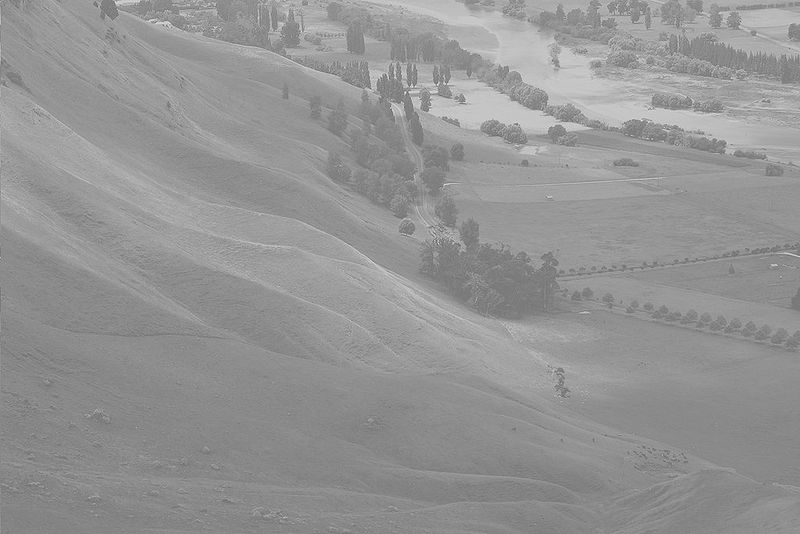
\includegraphics[scale=0.16]{images/histo01.jpg}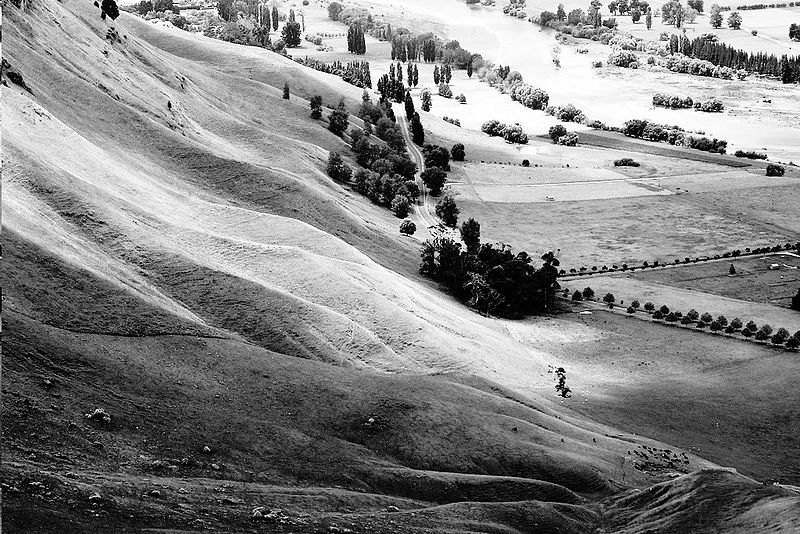
\includegraphics[scale=0.16]{images/histo03.jpg}} 
\end{center}
\begin{center}
{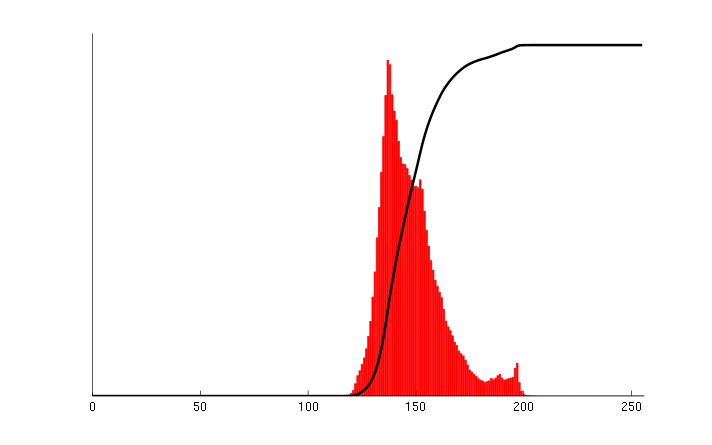
\includegraphics[scale=0.16]{images/histo02.png}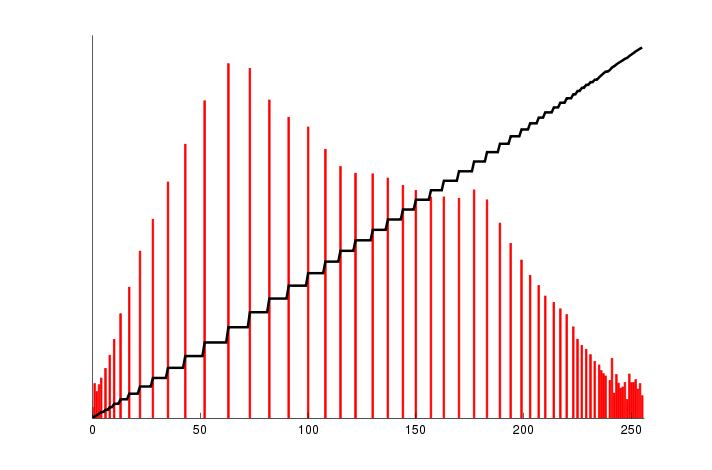
\includegraphics[scale=0.16]{images/histo04.png}} 
\end{center}
\caption{Résultat de l'Algorithme d'égalisation de l'histogramme}
(Source : Wikipédia)
\end{figure}

\subsection{Transformations géométriques}
Le résultat d'une transformation géométrique (rotation, transformations
affines, etc.) aboutit généralement à ce que les pixels de l'image
d'origine n'aient plus des coordonnées entières.

\paragraph{Inteprolation d'intensité} L'interpolation permet de déduire
la couleur des positions entières à partir des positions non entières
connues.

Exemple : Plus proches voisins, bilinéaire, bicubique, par convolution.

\paragraph{Convolution 1D}
$$(f * g)(x) = \int_{-\infty}^{+\infty}f(x-t) g(t) dt$$

\paragraph{Convolution 2D}
Soit $g$ une fonction telle que $\int_{\Bbb{R}^2}g(x,y)dxdy=1$.
On définit l'image traitée par convolution:
$$I_{\text{convol}} = I(x,y) * g(x, y) = \int_{\Omega}g(x - a, y -b) I(a,b) da db$$

L'influence des voisins sur le résultat en une position donnée va donc
dépendre du noyau de convolution $g$ utilisé. Cela permet de lisser mais
peut aussi induire du flou.

Ex : Noyau moyenneur, gaussienne, flou de bougé, etc.

\subparagraph{Remarque} Pour débruiter, un filtre médian est plus
efficace qu'un filtre moyenneur.

\section{Dérivées, opérateurs, discrétisation}
Principe: Voir une image non plus comme un tableau mais comme une fonction
$f(x,y) \in [0, 255]$


\subsection{Opérateurs usuels}

\paragraph{Dérivées partielles}
On peut considérer les dérivées partielles de l'image :
$\vert \frac{\partial f}{\partial x} \vert$ et $\vert \frac{\partial f}{\partial y} \vert$

\subparagraph{Interprétation} Une dérivée partielle grande indique une forte
variation selon la direction considérée $\longrightarrow$ permet de
détecter des contours mais dans une seule direction.

\paragraph{Gradient} Le gradient de $f$ est un champ de vecteurs:
$$\vec{\text{grad}} = \nabla f =
\left(\frac{\partial f}{\partial x}, \frac{\partial f}{\partial y} \right)$$

\subparagraph{Interprétation} Le gradient en une position donne la direction
est l'intensité de la plus forte variation autour de la position. Le
vecteur est dirigé vers les valeurs fortes. On peut donc aussi détecter
les contours, en considérant sa norme.

\paragraph{Laplacien} Le laplacien de $f$ est un champ de scalaire:
$$\Delta f = \frac{\partial^2 f}{\partial x^2} + \frac{\partial^2 f}{\partial y^2}$$

\paragraph{Divergence} La divergence d'un ensemble de vecteurs
$w = (w_1, \dots w_n)$ donne une information scalaire sur la variation
du volume autour du point.
$$\text{div} w = \frac{\partial w_1}{\partial x_1} + \dots + \frac{\partial w_n}{\partial x_n} = \nabla \cdot w$$

\paragraph{Rotationnel} 
Le rotationnel est un champ de vecteurs.
[À compléter, éventuellement,
pour ceux qui ont du temps, et du courage, ou une quelconque autre motivation]

\subsection{Équation aux dérivées partielles}
\paragraph{Définition} Une équation aux dérivées partielles (EDP) est un
système d'équations faisant intervenir les dérivées partielles de fonctions
qui sont les inconnues.

\paragraph{Équation de la chaleur} EDP décrivant l'évolution de la
température $T(x,y,t)$ en l'absence de contraintes extérieures.
$$\forall (x,y) \in \Omega \frac{\partial T(x,y,t)}{\partial t} = \Delta T(x,y,t)
\quad\text{et}\quad T(x,y,0) = T_0$$

Attention le laplacien ne concerne que l'espace, ie les coordonnées $x$ et $y$

En image, la température initiale $T_0$ est donnée par $f(x,y)$.

\subparagraph{Diffusion isotrope} Diffusion sans orientation préférentielle.

La diffusion induite par l'équation de la chaleur appliquée à une image
est isotrope. Au bout d'un certain temps, l'image devient flou puis s'unifie
(homogénéisation de la température).

\paragraph{Résolution 1D} La solution de l'équation de la chaleur en 1D
$$ \frac{\partial u(x,t)}{\partial t} = \frac{\partial^2 u(x,t)}{\partial x ^2}
\quad\text{avec}\quad u(x,0) = u_0(x)$$
est $$u(x,t) = G_{\sqrt{2t}}(x,t) * u_0(x)$$
où $G_{a}$ est une gausienne d'écart type $a$.

\paragraph{Résolution 2D} De même, la solution de l'équation de la
chaleur en 2D
$$ \frac{\partial u(x,y,t)}{\partial t} = \Delta u(x,y,t)
\quad\text{avec}\quad u(x,y,0) = u_0(x,y)$$
est $$u(x,y,t) = G_(x,t,\sigma (t)) * u_0(x,y)$$
où $G_(x,t,\sigma (t))$ est une gausienne d'écart type $\sigma$
proportionnel à $t$.

\paragraph{Application à une image}La diffusion est isotrope, elle floute
donc toute l'image, sans s'arrêter aux contours. On utilise donc la divergence
pour obtenir une diffusion non-linéaire \emph{anisotrope} d'une image $I$.
$$\frac{\partial I}{\partial t} = \text{div} \left(f(x,y)\nabla I \right)$$
\begin{itemize}
\item $f$ petit $\to$ divergence faible $\to$ peu de variation au cours
du temps.
\item $f$ grand $\to$ divergence grande $\to$ diffusion importante
\end{itemize}
Ainsi les zones unies sont homogénéisées mais les contours sont conservés.

\paragraph{Autre diffusion non linéaire}Perona-Malik, diffuse selon la
norme du gradient.

\subsection{Discrétisation}
Les dérivées partielles ne sont utilisables qu'en continu.

En continu, en trouve une solution analytique.
En discret, on construit une solution, étape après étape.

\paragraph{Différences finies} On peut remplacer les dérivées partielles
par des différences finies. Pour une image décrite par une grille de pixel,
on a $I(i,j) = u(i\Delta x, j\Delta y)$ où $I$ est discrète et $u$ continue,
$\Delta x$ et $\Delta y$ sont des pas de discrétisation.
La dérivée partielle peut alors être décrite par différentes formules
$$\frac{I(j + 1,j) - I(i,j)}{\Delta x} \quad \text{(Schéma arrière)}$$
ou
$$\frac{I(j - 1,j) - I(i,j)}{-\Delta x} \quad \text{(Schéma avant)} $$
ou
$$\frac{I(j + 1,j) - I(i - 1,j)}{2\Delta x} \quad \text{(Schéma centré)} $$

\subparagraph{Remarque} Généralement pour les images, on prend
$\Delta x = \Delta y = 1$.

\subparagraph{Conditions aux bords} Ce système pose la question des
conditions aux bords. Une solution est de copier en miroir les bords pour
prolonger l'image.

\subparagraph{Sensibilité au bruit} Ce type de différenciation est très
sensible au bruit. On peut augmenter la robustesse en filtrant avant de
différencier (filtre linéaire, moyenneur ou gaussien par exemple).

\paragraph{EDP} Avec cette différenciation discrète, on peut re-résoudre
l'EDP d'une variable 1D discrète
$\frac{\partial v}{\partial t} = \alpha \frac{\partial^2 v}{\partial x ^2}$.
On trouve l'approximation $u$ de $v$, pour un pas $\Delta t$
$$u_k^{n+1} = (1 - 2r)u_k^n + r(u_{k+1}^n + u_{k-1}^n)
\quad\text{avec}\quad r = \alpha \frac{\Delta t}{\Delta x^2}$$
et où $u_k^n = u(k\Delta x, n\Delta t)$ est la variable à l'étape $n$,
translatée de $k$ pas sur $x$.

\subsection{Stabilité d'un schéma numérique}
\paragraph{Analyse} Comment choisir $\Delta x$ et $\Delta t$ ? Le choix
lors de la discrétisation va reposer sur la notion de \emph{consistance}
et de \emph{stabilité}.

\paragraph{Schéma convergent} Il y a convergence si, quand $\Delta x \to 0$
et $\Delta t \to 0$, $(k\Delta x, n\Delta t) \to (x,t)\ \Rightarrow\ u_k^n \to v(t,x)$

\paragraph{Schéma consistant} Un schéma convergent est consistant si,
lorsque les pas tendent vers $0$, l'erreur de discrétisation tend vers $0$ ie
les approximations discrètes des dérivées tendent vers les dérivées continues.

\paragraph{Stabilité}Un processus de calcul séquentiel est stable si les
erreurs d'arrondis ne s'amplifient pas lors de la progression des calculs.
$$\|u^{n+1} \| \le K\|u^0\|$$

\subparagraph{Exemple} En considérant la norme $\|u^n\| = \sup_k{|u_k^n|}$,
notre schéma précédent est stable pour $r \le \frac{1}{2}$

\subparagraph{Méthode générale}La méthode de Fourier permet de prouver
la stabilité d'un processus.

\paragraph{Explicite/Implicite} Un schéma est explicite si on peut écrire
$u_k^{n+1}$ en fonction de $u_i^n$ pour un certain $i$. Il est implicite
sinon.

\section{Restauration d'images}
On considère trois types de régularisation: débruitage, déconvolution
(«défloutage») et inpainting (ou désocclusion).

\paragraph{Modélisation mathématique} La dégradation d'une image $f_0$
inconnue en une image $f$ observée se traduit par $f = \mathcal{R} f_0 + \eta$
où $\mathcal{R}$ est l'opérateur représentant la dégradation déterministe
(ex: convolution avec une gaussienne, opérateur de masquage) et $\eta$ est
une image aléatoire, le bruit.

\subparagraph{Bruit} On suppose que $\eta$ décrit un bruit blanc, ie
que toutes les fréquences ont la même importance dans le processus aléatoire.
Généralement, on prend un bruit blanc gaussien, la loi de probabilité des
fréquences est alors une gaussienne.

\subsection{Régularisation}
\paragraph{Score de régularité} Il existe une infinité de $\eta$ aboutissant
à une image initiale $f_0$. On sait cependant que l'image initiale était
«lisse». On a donc besoin de mesurer la régularité. Souvent, on utilise la
norme du gradient $\phi (u) = \int_\Omega \|\nabla u(x) \|^2d\Omega$.

\paragraph{Modélisation} On aboutit à la résolution du problème:
$$\mathcal{R}u \ \text{proche de}\  f \qquad\text{ET}\qquad u\  \text{régulière}$$
Une modélisation possible est alors
$$ \|f - \mathcal{R}u\|^2_{\mathscr{L}^2} =
\int_\Omega \left( f(x) - \mathcal{R} u(x) \right)^2 d\Omega \quad\text{petit}$$
$$ \|\nabla u\|^2_{\mathscr{L}^2} =
\int_\Omega \|\nabla u(x) \|^2d\Omega \quad\text{petit}$$

\paragraph{Régularisation de Tikhonov} On cherche $u$ telle que
$$ \inf_u
\underbrace{\int_\Omega \left( f(x) - \mathcal{R} u(x) \right)^2 d\Omega}_{\text{Terme de fidelité}}
+ \lambda \underbrace{\int_\Omega \|\nabla u(x) \|^2d\Omega}_{\text{Régularisation}}$$

\subsection{Minimisation de fonctionnelle}

\paragraph{Méthodes locales} Depuis un point $x_0$ on construit une
suite de point avec une condition d'arrêt. Ex: Descente de gradient,
recuit simulé.

\paragraph{Méthodes globales} On cherche directement le minimum global.
Ex: Moindre carré, simplexe, algos génétiques.

\paragraph{Descente de gradient} On se déplace dans la direction opposé au
gradient, c'est la direction de la plus grande descente. On avance à un
pas proportionnel au gradient.

\subparagraph{Limites de l'algo} On ne converge que vers un minimum local
dépendant du point de départ. Dans les zones «plates», le gradient est
faible et donc l'algo lent.

\paragraph{Image} Pour adapter la méthode de descente de gradient aux
images on passe par la dérivée de Gâteaux.

\subparagraph{Dérivée de Gâteaux} La dérivée de Gâteaux de $J$ au point
$u$ dans la direction $\phi$ est définie par
$$\lim_{\epsilon \to 0} \frac{J(u + \epsilon \phi) - J(u)}{\epsilon}$$

On cherche $\inf_u J(u)$. Après calculs, on trouve une EDP:
$$\frac{\partial F}{\partial u(x,y)}(x, y, u(x,y),\nabla u(x,y))
- \sum_{i=1}^n \frac{\partial}{\partial x_i}
(\frac{\partial F}{\partial \xi_i}(x, y, u(x,y),\nabla u(x,y))) = 0$$
où $\frac{\partial F}{\partial \xi_i}$ est la dérivée partielle par
rapport à la i\ieme composante de $\nabla u (x,y)$.
C'est l'\emph{Équation d'Euler-Lagrange} associée au problème d'optimisation.

\subsection{Débruitage}
\paragraph{Régularisation de Tikhonov} En utilisant l'EDP précédente,
on montre qu'il faut résoudre l'EDP $u(x,y) -f(x,y) -\lambda \nabla u(x,y) = 0$
pour résoudre le problème de minimisation.

\paragraph{Descente de gradient} La formule de descente de gradient devient
$$\frac{\partial u(x,t)}{\partial t} = -\left(\frac{\partial F}{\partial u(x,y)}
- \sum_{i=1}^n \frac{\partial}{\partial x_i} (\frac{\partial F}{\partial \xi_i})\right)$$

\paragraph{Discrétisation} Au final à chaque étape de la descente on a
$$u_{i,j}^{n+1} = u_{i,j}^n - \Delta t \left(\frac{\partial F}{\partial u(x,y)}
- \sum_{i=1}^n \frac{\partial}{\partial x_i} (\frac{\partial F}{\partial \xi_i})\right)$$

\paragraph{Observation} La courbe d'énergie (ie le terme régularisant)
est bien décroissant et converge vers 0. L'énergie est convexe donc ne
dépend pas de l'initialisation, prendre $u^0 = f$ accélère la convergence.

\paragraph{Diffusion linéaire} L'opérateur laplacien $\nabla$ lisse
de manière isotrope et altère donc trop les contours. On transforme
l'équation pour moins pénaliser les gradients forts grâce à une fonction
$\Psi$ adaptée:
$$ J(u) =
\underbrace{\int_\Omega \left( u(x) -f(x) \right)^2 d\Omega}_{\text{Terme de fidelité}}
+ \lambda \underbrace{\int_\Omega \Psi{\|\nabla u(x) \|}d\Omega}_{\text{Régularisation}}$$

\paragraph{Nouvelle descente de gradient}
$$\frac{\partial u}{\partial t} = 2(f - u) + \lambda \text{div}\left( \frac{\Psi'(\|\nabla u\|)}{\|\nabla u\|} \nabla u\right)$$
Avec par exemple: $\Psi(x) = \sqrt{\varepsilon + x^2} \xrightarrow[\varepsilon\to 0]{} \vert x \vert$

\subparagraph{Autres méthodes de débruitage} Non-Local Means et BM3D.

\subsection{Défloutage}
\paragraph{Adjoint} On définit l'adjoint $\mathcal{R}^*$ de $\mathcal{R}$
par  $<\mathcal{R}f \vert g> = <f \vert \mathcal{R}^* g>$.

\paragraph{$\mathcal{R} \neq$ Id} Si on considère la condition
$\lim_{\epsilon \to 0} \frac{J(u + \epsilon \phi) - J(u)}{\epsilon}$
alors il suffit de prendre $\phi = -2\mathcal{R}^*(\mathcal{R} u -f)$
pour avoir la convergence.

\subparagraph{Nouvelle descente de gradient}
$$\frac{\partial u}{\partial t} = 2\mathcal{R}^* f - 2 \mathcal{R}^*\mathcal{R} u$$

\paragraph{Déconvolution} Ici, $\mathcal{R} u = G_\sigma * u$. On peut alors
montrer que $\mathcal{R}^* = \mathcal{R}$

\subsection{Inpainting}
\paragraph{Descente de gradient} En précisant que l'on a un terme de régularité
($\lambda \neq 0$) on aboutit à la descente de gradient:
$$\frac{\partial u}{\partial t} = 2\mathcal{R}^* f - 2 \mathcal{R}^*\mathcal{R} u
+ \lambda \text{div}\left( \frac{\Psi'(\|\nabla u\|)}{\|\nabla u\|} \nabla u\right)$$
On peut aussi prouver que $\mathcal{R}^* = \mathcal{R}$.

\paragraph{Autre méthode} Le copier-coller.

\section{Segmentation}
\subsection{Seuillage d'histogramme}
\paragraph{Principe} On sépare les pixel de l'image selon que leur valeur
est au-dessus ou en dessous d'un certain seuil. On crée ainsi $k+1$ classes
en choisissant $k$ seuils.

\paragraph{Méthode d'Otsu} Seuillage d'histogramme où l'on minimise la
variance intra-classe.

\paragraph{Seuillage par classification bayésienne} On approxime
l'histogramme par un mélange de gaussiennes.

\subsection{Algo K-means}
\paragraph{Principe} Permet une classification en $k$ classes dans un
espace de dimension $n$. Si $n=1$ on a une image en niveaux de gris, $n=3$
une image en couleur.
\begin{itemize}
\item{Init} On initialiase $k$ graines aléatoires.
\item{Boucle} Jusqu'à convergence
\begin{itemize}
\item{Classification} Pour chaque pixel, on trouve la graine $i$ ma plus
proche. On étiquette ce pixel avec $i$.
\item{Équilibrage} On calcule le barycentre de chaque classe, ils deviennent
les nouvelles graines.
\end{itemize}
\end{itemize}

\subparagraph{Remarque}Pas de propriété sur la connexité.

\paragraph{Limites} Choix du nombre de classe et sensibilité à l'initialisation.

\paragraph{Variante} Algorithme des Fuzzy c-means. L'appartenance d'un
pixel à une classe est remplacé par une pondération de l'appartenance à
chacune des classes.

\paragraph{Autre méthode} Sélection récursive d'histogramme.

\subsection{Limites algos globaux} Des zones claires mais faiblement éclairées
seront dans la même classe que des zones sombres fortement éclairées.
Choisir une approche plus locale, en seuillant par région, ne suffit pas
car certaines zones ont un histogramme monomodal qui sera mal interprété.

\subsection{Region growing}

\paragraph{Principe} On part d'un ensemble de graines. On étend la zone
(classe) aux voisins en limitant l'écart-type de la classe à un seuil.

\paragraph{Avantages et limites}Implémentation rapide mais sensible aux
choix des graines, aux parcours des frontières des classes et au seuil.

\subsection{Split and merge}

\paragraph{Principe} On fonctionne en deux étapes : \emph{Split}, où on
partitionne l'image en sous-régions tant que la région n'est pas «homogène»
($\to$ graphe d'adjacence), et \emph{Merge}, où on regroupe les régions
voisines du graphes tant qu'elles sont homogènes.

\paragraph{Avantages et limites} Méthode hybride locale et globale mais
sensible au choix du seuil du critère d'homogénéité, à l'ordre de parcours.
Par ailleurs la segmentation finale présente des structures carrées.

\subsection{Méthode markovienne}
[Basé sur les probabilités et le recuit simulé]
\subsection{Graph-Cuts}
\subsection{Détecteur de Canny}

[Seuillage par la norme du gradient sur l'image lisser.]
\subsection{Segmentation par contours actifs}

[Minimiser le contour, favoriser une courbe régulière, fonctionne par
descente de gradient]
[Utilise le Level-Set pour permettre, entre autre des changement de
topologie. Extraction du niveau 0 par interpolation.]

\section{Transformée de Fourier}
\subsection{Transformée 1D}
\paragraph{Principe} On peut représenter un signal $f(x)$ par une
somme dénombrable de sinus/cosinus:
$$f(x) = \sum_{n = -\infty}^{+ \infty} c_n(f)e^{\imath 2\pi \frac{n}{T}}
\quad\text{avec}\quad c_n(f) = \frac{1}{T}\int_{-T/2}^{T/2} f(t) e^{-\imath 2\pi \frac{n}{T}t} $$
où $T$ est la période et $c_0(f)$ la moyenne de $f$

\paragraph{Transformée de Fourier 1D}
\subsection{Transformée 2D et 2D discrète}
\subsection{Transformée sur des images}

\end{document} 

